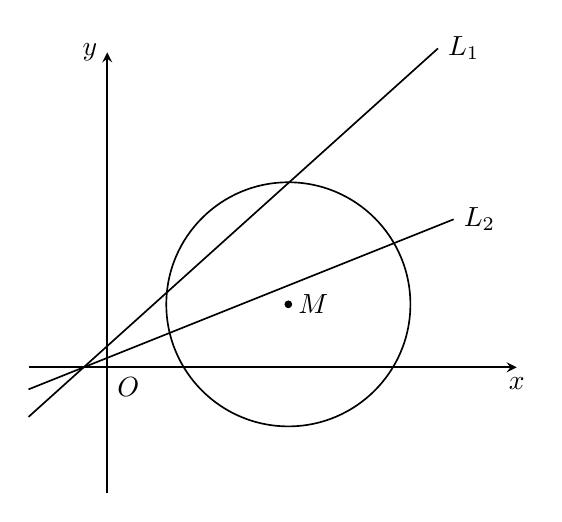
\begin{tikzpicture}[line width=.6pt, >=stealth, font=\normalsize]
  % axes
  \draw[->] (-1.6,0) -- (4.6,0) node[below] {$x$};
  \draw[->] (-0.6,-1.6) -- (-0.6,4.0) node[left] {$y$};
  \node[below right] at (-0.6,0) {$O$};
  % L1 (upper, steeper in schematic) and L2 (lower), intersect near origin
  \draw (-1.6,-.63) -- (3.6,4.05) node[right] {$L_{1}$};
  \draw (-1.6,-.28) -- (3.8,1.88) node[right] {$L_{2}$};
  % moving circle intersecting both lines in two points each
  \draw (1.7,.8) circle (1.55);
  \fill (1.7,.8) circle (1.4pt) node[right] {$M$};
\end{tikzpicture}
